\chapter{Artificial neural networks}\label{ann_chapter}
    Artificial neural networks (ANN) are a large class of models and learning methods that are in part inspired by biological neural networks and have widespread applications in many different fields.
    
    \section{Components of an artificial neural network}
        Basically, an artificial neural network consists of a large number of basic computing units (artificial neurons) that are connected to each other. Typically, artificial neurons are aggregated into layers. Each unit takes a number of inputs (possibly the outputs of other units) and produces a single value. This complex network of artificial neurons, where each connection can transmit a signal from a unit to another, allows to perform complex computations \cite[82]{Mitchell}.
        
        Formally, a single neuron is a mathematical function which transforms one or more real-value inputs in a single real-value output. It has two components:
        \begin{description}
            \item[Propagation function] It is a function which receives data input of other neurons and returns a single real-value output. A very popular propagation function is the weighted sum of the multiplication of the input of each neuron by the weight associated with the connection between the two units. Formally:
            \[net_j = \sum_{i=1}^{P}\left(o_i \cdot w_{i,j}\right)\]
            where \(o_1, o_2, \dots, o_P\) are the data input of other neurons, \(w_{i,j}\) the weights associated with the connections between the input neurons and the current one, and \(net_j\) the single output of the propagation function (also called network input).
            \item[Activation function] It is responsible for deciding whether a neuron should be activated or not --- i.e., whether the information that the neuron is receiving is relevant or should be ignored. Formally, it takes as input the network input \(net_j\) and the returned value will be the output of the neuron:
            \[o_j = \sigma\left(net_j\right)\]
            The simplest activation function is binary --- i.e., either the information is relevant or not. However, for most practical problems, activation functions should be bounded, monotonic and smooth (continuously differentiable). A very popular example is the logistic function: \(\sigma\left(net_j\right) = \frac{1}{1+e^{-net_j}}\).
        \end{description}
        See figure \ref{neuron_data_processing} for a visual representation of the data processing of a unit of an artificial neural network.
        
        \begin{figure}
    \centering
    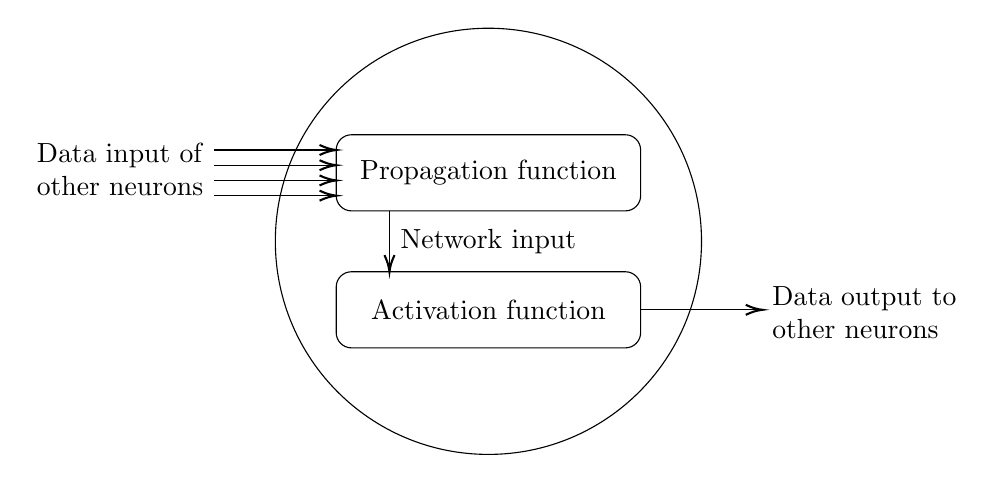
\begin{tikzpicture}[x=0.55pt,y=0.55pt,yscale=-1,xscale=1]
        %uncomment if require: \path (0,300); %set diagram left start at 0, and has height of 300
        
        %Shape: Circle [id:dp16703115491619047] 
        \draw   (155,150) .. controls (155,72.68) and (217.68,10) .. (295,10) .. controls (372.32,10) and (435,72.68) .. (435,150) .. controls (435,227.32) and (372.32,290) .. (295,290) .. controls (217.68,290) and (155,227.32) .. (155,150) -- cycle ;
        %Rounded Rect [id:dp968097124870297] 
        \draw   (195,90) .. controls (195,84.48) and (199.48,80) .. (205,80) -- (385,80) .. controls (390.52,80) and (395,84.48) .. (395,90) -- (395,120) .. controls (395,125.52) and (390.52,130) .. (385,130) -- (205,130) .. controls (199.48,130) and (195,125.52) .. (195,120) -- cycle ;
        %Rounded Rect [id:dp48825970598888957] 
        \draw   (195,180) .. controls (195,174.48) and (199.48,170) .. (205,170) -- (385,170) .. controls (390.52,170) and (395,174.48) .. (395,180) -- (395,210) .. controls (395,215.52) and (390.52,220) .. (385,220) -- (205,220) .. controls (199.48,220) and (195,215.52) .. (195,210) -- cycle ;
        %Straight Lines [id:da28699213799346746] 
        \draw    (230,130) -- (230,168) ;
        \draw [shift={(230,170)}, rotate = 270] [color={rgb, 255:red, 0; green, 0; blue, 0 }  ][line width=0.75]    (10.93,-3.29) .. controls (6.95,-1.4) and (3.31,-0.3) .. (0,0) .. controls (3.31,0.3) and (6.95,1.4) .. (10.93,3.29)   ;
        
        %Straight Lines [id:da4660434658597914] 
        \draw    (115,90) -- (193,90) ;
        \draw [shift={(195,90)}, rotate = 180] [color={rgb, 255:red, 0; green, 0; blue, 0 }  ][line width=0.75]    (10.93,-3.29) .. controls (6.95,-1.4) and (3.31,-0.3) .. (0,0) .. controls (3.31,0.3) and (6.95,1.4) .. (10.93,3.29)   ;
        
        %Straight Lines [id:da9228038405838919] 
        \draw    (115,100) -- (193,100) ;
        \draw [shift={(195,100)}, rotate = 180] [color={rgb, 255:red, 0; green, 0; blue, 0 }  ][line width=0.75]    (10.93,-3.29) .. controls (6.95,-1.4) and (3.31,-0.3) .. (0,0) .. controls (3.31,0.3) and (6.95,1.4) .. (10.93,3.29)   ;
        
        %Straight Lines [id:da7128529944980109] 
        \draw    (115,110) -- (193,110) ;
        \draw [shift={(195,110)}, rotate = 180] [color={rgb, 255:red, 0; green, 0; blue, 0 }  ][line width=0.75]    (10.93,-3.29) .. controls (6.95,-1.4) and (3.31,-0.3) .. (0,0) .. controls (3.31,0.3) and (6.95,1.4) .. (10.93,3.29)   ;
        
        %Straight Lines [id:da21112944427932812] 
        \draw    (115,120) -- (193,120) ;
        \draw [shift={(195,120)}, rotate = 180] [color={rgb, 255:red, 0; green, 0; blue, 0 }  ][line width=0.75]    (10.93,-3.29) .. controls (6.95,-1.4) and (3.31,-0.3) .. (0,0) .. controls (3.31,0.3) and (6.95,1.4) .. (10.93,3.29)   ;
        
        %Straight Lines [id:da7928692563036984] 
        \draw    (395,195) -- (473,195) ;
        \draw [shift={(475,195)}, rotate = 180] [color={rgb, 255:red, 0; green, 0; blue, 0 }  ][line width=0.75]    (10.93,-3.29) .. controls (6.95,-1.4) and (3.31,-0.3) .. (0,0) .. controls (3.31,0.3) and (6.95,1.4) .. (10.93,3.29)   ;
        
        
        % Text Node
        \draw (53,103) node  [align=left] {Data input of\\other neurons};
        % Text Node
        \draw (295,105) node  [align=left] {Propagation function};
        % Text Node
        \draw (295,195) node  [align=left] {Activation function};
        % Text Node
        \draw (295,150) node  [align=left] {Network input};
        % Text Node
        \draw (542,197) node  [align=left] {Data output to\\other neurons};
    \end{tikzpicture}
    \caption{Data processing of a neuron.}
    \label{neuron_data_processing}
\end{figure}
    
        To sum up, neural networks are sets of neurons organized in layers. They perform tasks by extracting linear combinations of the input features and modelling the target as a nonlinear function of these derived features \cite[389]{Hastie}.
    \section{Feed-forward neural networks}
        Feed-forward neural networks consist of neurons organized in layers (one input layer, one output layer, and a number of hidden layers), where each neuron in one layer is directly connected to all the neurons of the next layer. In other words, the output of every layer --- i.e., the set containing the output of each neuron of the layer --- serves as input for the next layer.
        
        Here is the basic notation used to formally describe how a feed-forward neural network works \cite[269--270]{Shalev-Shwartz}:
        \begin{itemize}
            \item \(X_1,X_2,\dots,X_N\) are the \(N\) features representing the input vector \(X\). The \(M\) components of the output vector \(\hat{Y}\) are \(\hat{Y}_1,\hat{Y}_2,\dots,\hat{Y}_M\).
            \item \(L\) is the number of layers (the input layer is not taken into account). \(P^t\) is the number of nodes belonging to the \(t\)-th layer (\(P^0=N\) and \(P^L=M\)).
            \item \(v_{i}^{t}\) denotes the \(i\)-th neuron of the \(t\)-th layer.
            \item \(w_{i,j}^{t}\) denotes the weight associated with the connection between the \(i\)-th neuron of layer \(t-1\) and the \(j\)-th neuron of layer \(t\) --- i.e., the connection between \(v_{i}^{t-1}\) and \(v_{j}^{t}\). \(b_{j}^{t}\) denotes the bias term associated with the \(v_{j}^{t}\).
            \item \(net_{i}^{t}\) and \(o_{i}^{t}\) are, respectively, the network input and the output of the neuron \(v_{i}^{t}\).
            \item \(\sigma^{t}\) denotes the activation function used in each neuron belonging to the \(t\)-th layer of the feed-forward neural network.
        \end{itemize}
        
        Suppose that the outputs at layer \(t-1\) have already been computed (with \(P^{0} = N\) and \(o_{1}^{0}=X_1, o_{2}^{0}=X_2,\dots, o_{N}^{0}=X_N\)). Then, the outputs at layer \(t\) can be calculated as follows:
        \[net_{j}^{t} = \sum_{i=1}^{P^{t-1}}w_{i,j}^{t} \cdot o_{i}^{t-1} + b_{j}^{t}\]
        \[o_{j}^{t} = \sigma^{t}\left(net_{j}^{t}\right)\]
        The propagation function is a linear combination of the inputs --- i.e., it is a weighted sum of the outputs of the neurons belonging to the previous layer --- and the activation function is a nonlinear function of this derived feature.
        
        \begin{figure}
    \centering
    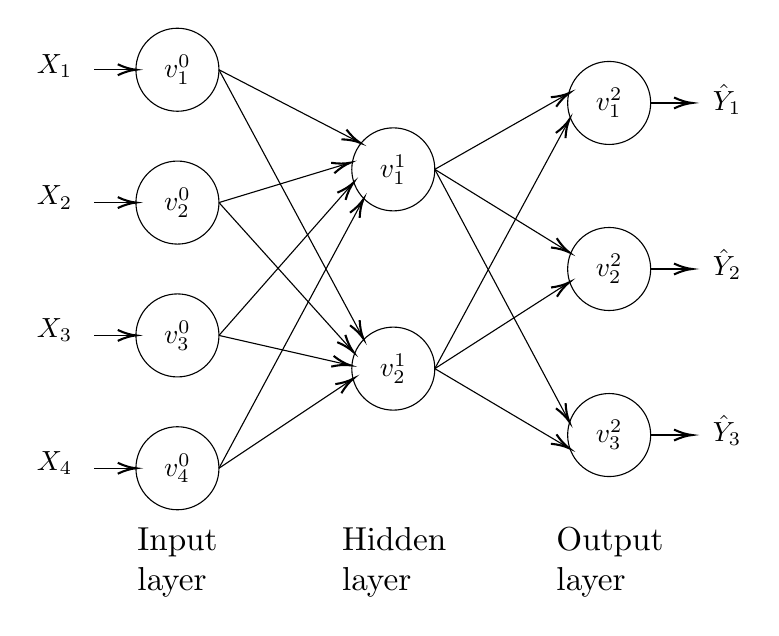
\begin{tikzpicture}[x=0.6pt,y=0.6pt,yscale=-1,xscale=1]
        %Flowchart: Connector [id:dp19821829949297887] 
        \draw   (65,30) .. controls (65,16.19) and (76.19,5) .. (90,5) .. controls (103.81,5) and (115,16.19) .. (115,30) .. controls (115,43.81) and (103.81,55) .. (90,55) .. controls (76.19,55) and (65,43.81) .. (65,30) -- cycle ;
        %Straight Lines [id:da7954557592474568] 
        \draw    (115,30) -- (198.22,73.08) ;
        \draw [shift={(200,74)}, rotate = 207.37] [color={rgb, 255:red, 0; green, 0; blue, 0 }  ][line width=0.75]    (10.93,-3.29) .. controls (6.95,-1.4) and (3.31,-0.3) .. (0,0) .. controls (3.31,0.3) and (6.95,1.4) .. (10.93,3.29)   ;
        
        %Straight Lines [id:da5247225635420859] 
        \draw    (115,30) -- (201.05,190.24) ;
        \draw [shift={(202,192)}, rotate = 241.76] [color={rgb, 255:red, 0; green, 0; blue, 0 }  ][line width=0.75]    (10.93,-3.29) .. controls (6.95,-1.4) and (3.31,-0.3) .. (0,0) .. controls (3.31,0.3) and (6.95,1.4) .. (10.93,3.29)   ;
        
        %Straight Lines [id:da46287226344247623] 
        \draw    (115,110) -- (192.09,86.58) ;
        \draw [shift={(194,86)}, rotate = 523.1] [color={rgb, 255:red, 0; green, 0; blue, 0 }  ][line width=0.75]    (10.93,-3.29) .. controls (6.95,-1.4) and (3.31,-0.3) .. (0,0) .. controls (3.31,0.3) and (6.95,1.4) .. (10.93,3.29)   ;
        
        %Straight Lines [id:da10799882710691722] 
        \draw    (115,190) -- (194.68,99.5) ;
        \draw [shift={(196,98)}, rotate = 491.36] [color={rgb, 255:red, 0; green, 0; blue, 0 }  ][line width=0.75]    (10.93,-3.29) .. controls (6.95,-1.4) and (3.31,-0.3) .. (0,0) .. controls (3.31,0.3) and (6.95,1.4) .. (10.93,3.29)   ;
        
        %Straight Lines [id:da4456004059779004] 
        \draw    (115,270) -- (201.05,109.76) ;
        \draw [shift={(202,108)}, rotate = 478.24] [color={rgb, 255:red, 0; green, 0; blue, 0 }  ][line width=0.75]    (10.93,-3.29) .. controls (6.95,-1.4) and (3.31,-0.3) .. (0,0) .. controls (3.31,0.3) and (6.95,1.4) .. (10.93,3.29)   ;
        
        %Straight Lines [id:da39810869317669284] 
        \draw    (115,110) -- (194.66,198.51) ;
        \draw [shift={(196,200)}, rotate = 228.01] [color={rgb, 255:red, 0; green, 0; blue, 0 }  ][line width=0.75]    (10.93,-3.29) .. controls (6.95,-1.4) and (3.31,-0.3) .. (0,0) .. controls (3.31,0.3) and (6.95,1.4) .. (10.93,3.29)   ;
        
        %Straight Lines [id:da5777691196107136] 
        \draw    (115,190) -- (192.05,207.56) ;
        \draw [shift={(194,208)}, rotate = 192.84] [color={rgb, 255:red, 0; green, 0; blue, 0 }  ][line width=0.75]    (10.93,-3.29) .. controls (6.95,-1.4) and (3.31,-0.3) .. (0,0) .. controls (3.31,0.3) and (6.95,1.4) .. (10.93,3.29)   ;
        
        %Straight Lines [id:da9952648605104905] 
        \draw    (115,270) -- (194.34,217.11) ;
        \draw [shift={(196,216)}, rotate = 506.31] [color={rgb, 255:red, 0; green, 0; blue, 0 }  ][line width=0.75]    (10.93,-3.29) .. controls (6.95,-1.4) and (3.31,-0.3) .. (0,0) .. controls (3.31,0.3) and (6.95,1.4) .. (10.93,3.29)   ;
        
        %Straight Lines [id:da35658039205845227] 
        \draw    (245,90) -- (324.26,44.99) ;
        \draw [shift={(326,44)}, rotate = 510.41] [color={rgb, 255:red, 0; green, 0; blue, 0 }  ][line width=0.75]    (10.93,-3.29) .. controls (6.95,-1.4) and (3.31,-0.3) .. (0,0) .. controls (3.31,0.3) and (6.95,1.4) .. (10.93,3.29)   ;
        
        %Straight Lines [id:da9791877092679799] 
        \draw    (245,210) -- (325.05,61.76) ;
        \draw [shift={(326,60)}, rotate = 478.37] [color={rgb, 255:red, 0; green, 0; blue, 0 }  ][line width=0.75]    (10.93,-3.29) .. controls (6.95,-1.4) and (3.31,-0.3) .. (0,0) .. controls (3.31,0.3) and (6.95,1.4) .. (10.93,3.29)   ;
        
        %Straight Lines [id:da3601300378176867] 
        \draw    (245,210) -- (324.32,159.08) ;
        \draw [shift={(326,158)}, rotate = 507.3] [color={rgb, 255:red, 0; green, 0; blue, 0 }  ][line width=0.75]    (10.93,-3.29) .. controls (6.95,-1.4) and (3.31,-0.3) .. (0,0) .. controls (3.31,0.3) and (6.95,1.4) .. (10.93,3.29)   ;
        
        %Straight Lines [id:da9284525375768318] 
        \draw    (245,210) -- (324.28,256.98) ;
        \draw [shift={(326,258)}, rotate = 210.65] [color={rgb, 255:red, 0; green, 0; blue, 0 }  ][line width=0.75]    (10.93,-3.29) .. controls (6.95,-1.4) and (3.31,-0.3) .. (0,0) .. controls (3.31,0.3) and (6.95,1.4) .. (10.93,3.29)   ;
        
        %Straight Lines [id:da2356739692743225] 
        \draw    (245,90) -- (324.3,138.95) ;
        \draw [shift={(326,140)}, rotate = 211.69] [color={rgb, 255:red, 0; green, 0; blue, 0 }  ][line width=0.75]    (10.93,-3.29) .. controls (6.95,-1.4) and (3.31,-0.3) .. (0,0) .. controls (3.31,0.3) and (6.95,1.4) .. (10.93,3.29)   ;
        
        %Straight Lines [id:da2610075440778471] 
        \draw    (245,90) -- (325.06,240.23) ;
        \draw [shift={(326,242)}, rotate = 241.95] [color={rgb, 255:red, 0; green, 0; blue, 0 }  ][line width=0.75]    (10.93,-3.29) .. controls (6.95,-1.4) and (3.31,-0.3) .. (0,0) .. controls (3.31,0.3) and (6.95,1.4) .. (10.93,3.29)   ;
        
        %Flowchart: Connector [id:dp956277214202537] 
        \draw   (65,110) .. controls (65,96.19) and (76.19,85) .. (90,85) .. controls (103.81,85) and (115,96.19) .. (115,110) .. controls (115,123.81) and (103.81,135) .. (90,135) .. controls (76.19,135) and (65,123.81) .. (65,110) -- cycle ;
        %Flowchart: Connector [id:dp9721204392167134] 
        \draw   (65,190) .. controls (65,176.19) and (76.19,165) .. (90,165) .. controls (103.81,165) and (115,176.19) .. (115,190) .. controls (115,203.81) and (103.81,215) .. (90,215) .. controls (76.19,215) and (65,203.81) .. (65,190) -- cycle ;
        %Flowchart: Connector [id:dp9465269748932483] 
        \draw   (195,90) .. controls (195,76.19) and (206.19,65) .. (220,65) .. controls (233.81,65) and (245,76.19) .. (245,90) .. controls (245,103.81) and (233.81,115) .. (220,115) .. controls (206.19,115) and (195,103.81) .. (195,90) -- cycle ;
        %Flowchart: Connector [id:dp7248390077237111] 
        \draw   (195,210) .. controls (195,196.19) and (206.19,185) .. (220,185) .. controls (233.81,185) and (245,196.19) .. (245,210) .. controls (245,223.81) and (233.81,235) .. (220,235) .. controls (206.19,235) and (195,223.81) .. (195,210) -- cycle ;
        %Flowchart: Connector [id:dp8686198245718617] 
        \draw   (325,250) .. controls (325,236.19) and (336.19,225) .. (350,225) .. controls (363.81,225) and (375,236.19) .. (375,250) .. controls (375,263.81) and (363.81,275) .. (350,275) .. controls (336.19,275) and (325,263.81) .. (325,250) -- cycle ;
        %Flowchart: Connector [id:dp7424235612073783] 
        \draw   (325,150) .. controls (325,136.19) and (336.19,125) .. (350,125) .. controls (363.81,125) and (375,136.19) .. (375,150) .. controls (375,163.81) and (363.81,175) .. (350,175) .. controls (336.19,175) and (325,163.81) .. (325,150) -- cycle ;
        %Flowchart: Connector [id:dp5509872207216341] 
        \draw   (325,50) .. controls (325,36.19) and (336.19,25) .. (350,25) .. controls (363.81,25) and (375,36.19) .. (375,50) .. controls (375,63.81) and (363.81,75) .. (350,75) .. controls (336.19,75) and (325,63.81) .. (325,50) -- cycle ;
        %Flowchart: Connector [id:dp8479291224575998] 
        \draw   (65,270) .. controls (65,256.19) and (76.19,245) .. (90,245) .. controls (103.81,245) and (115,256.19) .. (115,270) .. controls (115,283.81) and (103.81,295) .. (90,295) .. controls (76.19,295) and (65,283.81) .. (65,270) -- cycle ;
        %Straight Lines [id:da7179799472210422] 
        \draw    (40,30) -- (63,30) ;
        \draw [shift={(65,30)}, rotate = 180] [color={rgb, 255:red, 0; green, 0; blue, 0 }  ][line width=0.75]    (10.93,-3.29) .. controls (6.95,-1.4) and (3.31,-0.3) .. (0,0) .. controls (3.31,0.3) and (6.95,1.4) .. (10.93,3.29)   ;
        
        %Straight Lines [id:da040628165924566306] 
        \draw    (40,110) -- (63,110) ;
        \draw [shift={(65,110)}, rotate = 180] [color={rgb, 255:red, 0; green, 0; blue, 0 }  ][line width=0.75]    (10.93,-3.29) .. controls (6.95,-1.4) and (3.31,-0.3) .. (0,0) .. controls (3.31,0.3) and (6.95,1.4) .. (10.93,3.29)   ;
        
        %Straight Lines [id:da047613112945486535] 
        \draw    (40,190) -- (63,190) ;
        \draw [shift={(65,190)}, rotate = 180] [color={rgb, 255:red, 0; green, 0; blue, 0 }  ][line width=0.75]    (10.93,-3.29) .. controls (6.95,-1.4) and (3.31,-0.3) .. (0,0) .. controls (3.31,0.3) and (6.95,1.4) .. (10.93,3.29)   ;
        
        %Straight Lines [id:da7076667926767186] 
        \draw    (40,270) -- (63,270) ;
        \draw [shift={(65,270)}, rotate = 180] [color={rgb, 255:red, 0; green, 0; blue, 0 }  ][line width=0.75]    (10.93,-3.29) .. controls (6.95,-1.4) and (3.31,-0.3) .. (0,0) .. controls (3.31,0.3) and (6.95,1.4) .. (10.93,3.29)   ;
        
        %Straight Lines [id:da991735367031057] 
        \draw    (375,50) -- (398,50) ;
        \draw [shift={(400,50)}, rotate = 180] [color={rgb, 255:red, 0; green, 0; blue, 0 }  ][line width=0.75]    (10.93,-3.29) .. controls (6.95,-1.4) and (3.31,-0.3) .. (0,0) .. controls (3.31,0.3) and (6.95,1.4) .. (10.93,3.29)   ;
        
        %Straight Lines [id:da2231985342302314] 
        \draw    (375,150) -- (398,150) ;
        \draw [shift={(400,150)}, rotate = 180] [color={rgb, 255:red, 0; green, 0; blue, 0 }  ][line width=0.75]    (10.93,-3.29) .. controls (6.95,-1.4) and (3.31,-0.3) .. (0,0) .. controls (3.31,0.3) and (6.95,1.4) .. (10.93,3.29)   ;
        
        %Straight Lines [id:da7456308816655278] 
        \draw    (375,250) -- (398,250) ;
        \draw [shift={(400,250)}, rotate = 180] [color={rgb, 255:red, 0; green, 0; blue, 0 }  ][line width=0.75]    (10.93,-3.29) .. controls (6.95,-1.4) and (3.31,-0.3) .. (0,0) .. controls (3.31,0.3) and (6.95,1.4) .. (10.93,3.29)   ;
        
        % Text Node
        \draw (90,30) node   {$v_{1}^0$};
        % Text Node
        \draw (90,110) node   {$v_{2}^0$};
        % Text Node
        \draw (90,190) node   {$v_{3}^0$};
        % Text Node
        \draw (90,270) node   {$v_{4}^0$};
        % Text Node
        \draw (220,90) node   {$v_{1}^1$};
        % Text Node
        \draw (220,210) node   {$v_{2}^1$};
        % Text Node
        \draw (350,250) node   {$v_{3}^2$};
        % Text Node
        \draw (350,150) node   {$v_{2}^2$};
        % Text Node
        \draw (350,50) node   {$v_{1}^2$};
        % Text Node
        \draw (16,28) node   {$X_{1}$};
        % Text Node
        \draw (16,107) node   {$X_{2}$};
        % Text Node
        \draw (16,187) node   {$X_{3}$};
        % Text Node
        \draw (16,267) node   {$X_{4}$};
        % Text Node
        \draw (421,48) node   {$\hat{Y}_{1}$};
        % Text Node
        \draw (421,147) node   {$\hat{Y}_{2}$};
        % Text Node
        \draw (421,247) node   {$\hat{Y}_{3}$};
        % Text Node
        \draw (90,326.5) node [scale=1.2] [align=left] {Input\\layer};
        % Text Node
        \draw (220.5,326.5) node [scale=1.2] [align=left] {Hidden\\layer};
        % Text Node
        \draw (350.5,326.5) node [scale=1.2] [align=left] {Output\\layer};
    \end{tikzpicture}
    \caption{Schematic of a single hidden layer, fully connected, feed-forward neural network.}
    \label{feedforward_nn}
\end{figure}

        
        A simple feed-forward neural network is represented in figure \ref{feedforward_nn}. The units in the middle layer are called hidden units because their output values are not directly observable. In general, there can be an arbitrary number of hidden layers and their outputs can be thought of as nonlinear transformations of the original inputs \(X_i\) \cite[393]{Hastie}.
        
    \section{Network training}
        The behavior of a neural network depends on the weights associated with each connection between neurons. These supervised algorithms learn how to perform various tasks by fitting the training data and adjusting weights associated to connections. In other words, given an input and the related output produced by the network, the algorithm takes the ideal output and adjusts the weights in order to produce a more accurate output the next time. In general, neural networks need a learning strategy --- i.e., an algorithm that:
        \begin{itemize}
            \item Uses training data to change the weights.
            \item Makes the model produce the desired output for a given input, thus allowing accurate predictions.
        \end{itemize}
        
        In order to training a neural network, one must choose the loss function and an optimizer, as described in section \ref{components_ml}. Moreover, it is also fundamental to choose the activation functions used in each layer.
        
        \subsection{Good practices for choosing activation and loss functions}
            In order to get good results with neural networks, many researchers have developed some best practices over the years (for example, see \cite{Simard}). Some of them have focused on the choice of activation and loss functions according to the type of problem being solved \cite[232--236]{Bishop}:
            \begin{itemize}
                \item For regression problems, it is common to have a single output neuron. The activation functions used in such neuron should be linear. Moreover, a good loss function is the sum-of-squares error
                \[L\left(x_1, x_2, \dots, x_n\right) = \frac{1}{n} \cdot \sum_{i=1}^{n}\left(\hat{y}_i - y_i\right)^{2}\]
                \item For binary classification problems, it is common to have a single output neuron, representing the probability associated with the positive class. Good outputs may be obtained using standard logistic sigmoid as activation function, and cross-entropy as loss function.
                \[\hat{Y}_j = \sigma^L\left(net_j^L\right) = \frac{1}{1+e^{-net_j^L}}\]
                \[L\left(x_1, x_2, \dots, x_n\right) = -\frac{1}{n} \cdot \sum_{i=1}^{n}\left[y_i \cdot ln\left(\hat{y}_i\right) + \left(1-y_i\right)\cdot ln\left(1-\hat{y}_i\right)\right]\]
                \item For multi-class classification --- where each input is assigned to one of \(K\) mutually exclusive classes --- it is common to have as many neurons in the last layer as the number of classes. Outputs of these neurons are often interpreted as a probability distribution over classes. Softmax outputs are usually a good choice and they are used together with the corresponding multi-class cross-entropy loss function.
                \[\hat{Y}_j = \sigma_j^L\left(net_1^L, net_2^L, \dots, net_K^L\right) = \frac{e^{net_j^L}}{\sum_{k=1}^{K}e^{net_k^L}}\]
                \[L\left(x_1, x_2, \dots, x_n\right) = -\frac{1}{n} \cdot  \sum_{i=1}^{n}\sum_{k=1}^{K}y_{ik} \cdot ln\left(\hat{y}_{ik}\right)\]
            \end{itemize}
        \subsection{Weights optimization using gradient information}
            Once the network is built and the error function chosen, one must define an algorithm that minimizes the loss function with respect to the weights.
            
            Since the error function \(L\) is a smooth continuous function, its global minimum --- and, in general, all the local minima --- is a stationary point and thus occurs at a point in which the gradient vanishes --- i.e. \(\nabla L\left(w\right) = 0\). The goal of the optimization algorithm is to find the vector \(w\) of weights which minimizes the loss function \(L\) --- i.e., the difference between the actual output of the network and the desired output.
            
            Being the loss function highly complex, a solution cannot be found in an analytic way. Instead, the optimization algorithm must use numerical methods. Many techniques used in literature involve starting with some carefully chosen weights and then moving step-by-step through the weight space
            \[w^{\left(r+1\right)} = w^{\left(r\right)} + \Delta w^{\left(r\right)}\]
            until the values converge. Specifically, one must choose both the direction and the size of the step.
            
            As of the direction, the most popular choice is to take steps proportional to the negative of the gradient \cite[240]{Bishop}: the idea is to move in the direction along which the loss function decreases the fastest. With regard to the step size --- or learning rate --- it cannot be too high or too low: if it is too high then the algorithm may miss minima or even diverge, if it is too low then the algorithm may take too long to converge or get stuck in non-optimal local minima.
            
            Unfortunately, minimizing the loss function is not an easy task. In fact, the loss function is highly nonlinear and nonconvex \cite[400]{Hastie}\cite[237]{Bishop}: it possesses many local minima, local maxima and saddle points. Therefore, many variants of the basic gradient descent algorithm have been studied for years. For example, the learning rate may be fixed or change over iterations. Also, the gradient might be stochastic --- i.e., computed approximately using only some random samples --- or it could be improved using momentum, which prevents excessive oscillations.
        \subsection{Back-propagation}
            Not only the loss function is highly nonconvex, but it is also unknown: the training dataset comprises only few examples. How can the gradient of such function be computed or approximated? Back-propagation is a computationally efficient technique for evaluating derivatives of the error function with respect to the weights (which are then used to adjust the weights of the network, thus obtaining outputs which are closer to the ideal ones), and it can be used with a wide variety of loss and activation functions. This method --- whose importance was not fully appreciated until a famous \citeyear{Rumelhart} paper by \citeauthor{Rumelhart} (see \cite{Rumelhart}) --- is called back-propagation because errors are propagated backward through the network.
            
            Formally, back-propagation aims at computing the partial derivatives \(\frac{\partial L}{\partial w}\) and \(\frac{\partial L}{\partial b}\) of the loss function \(L\) with respect to any weight \(w\) or bias \(b\) in the network. Computing partial derivatives is about understanding how changing the weights and biases in a network changes the value of the error function --- i.e., the difference between the actual and desired outputs.
            
            Back-propagation is merely a highly efficient application of the chain rule used in calculus\footnote{A formula for finding the derivative of a function with respect to any variable in the nested equation.} \cite[205]{Goodfellow}:
            \[\left(f \circ g\right)^{\prime}\left(x\right) = f^{\prime}\left(g\left(x\right)\right) \cdot g^{\prime}\left(x\right)\]
            
            Using such formula, one can easily derive the partial derivatives of the loss function with respect to weights and biases (there might be some issues if activation functions are discontinuous or not-differentiable). For example, given that
            \[net_{j}^{t} = \sum_{i=1}^{P^{t-1}}w_{i,j}^{t} \cdot o_{i}^{t-1} + b_{j}^{t}\]
            \[L\left(x_1, x_2, \dots, x_n\right) = \frac{1}{2n}\sum_{i=1}^{n}\left(\hat{y}_i - y_{i}\right)^{2}\]
            then
            \[\frac{\partial L}{\partial w_{i,j}^{t}} = \delta_{j}^{t} \cdot \frac{\partial net_{j}^{t}}{\partial w_{i,j}^{t}} = \delta_{j}^{t} \cdot o_{i}^{t-1}\]
            where the calculation of the term \(\delta_{j}^{t}\) is dependent on the values of the terms \(\delta_{1}^{t+1}, \delta_{2}^{t+1}, \dots, \delta_{P^{t+1}}^{t+1}\) related to the next layer\footnote{This is the origin of the name back-propagation: computation of the error term proceeds backwards.}:
            \[\delta_{j}^{t} = \frac{\partial \sigma_j^t}{\partial net_j^t}\sum_{i=1}^{P^{t+1}}w_{j,i}^{t+1}\delta_{i}^{t+1}\]
        \subsection{Issues in training neural networks}
            Most good practices in machine learning are guided by background knowledge and experimentation. Here are some important issues that one may face while dealing with training neural networks \cite[397--401]{Hastie}:
            \begin{itemize}
                \item When building a neural network, one must define the number of hidden units and layers (the number of input and output neurons is fixed by the problem statement). One should always keep in mind that on one hand adding layers improves the ability of the network to represent difficult functions, but on the other hand it generates additional local minima in which the optimization algorithm can get stuck. As of the number of neurons per layer, it corresponds to the number of free parameters of the model: according to the Ockham's razor, the goal is to have as few nodes as possible but as many as necessary.
                \item In order to search the weight space, optimization algorithms usually need values to start from: since the loss function is highly complex --- i.e., it has many local minima --- it is important to carefully choose the starting values, so that the optimization algorithm is likely to explore interesting regions of the space. A very simple but effective strategy is to initialize weights with small random values \cite[302]{Goodfellow}.
                \item Setting a good learning rate and the right optimization algorithm has significant impact on model performance \cite[306--310]{Goodfellow}. There exist a large number of optimization algorithms, and each of them adapts the learning rate in a different way: unfortunately, there is no single best algorithm \cite{Schaul}.
            \end{itemize}
    \section{Convolutional neural networks}
        Convolutional neural networks --- or CNNs --- are a category of artificial neural network for processing data that has a spatial structure --- i.e., a grid-like topology \cite[330]{Goodfellow}\cite{LeCunDeepLearning}. Typical examples of data used with a convolutional neural network are images, volumetric data (a common source of this kind of data is a CT scan\footnote{A technique that allows the user to see inside an object by combining many X-ray measurements taken from different angles.}) or discretized audio waves.
        
        Convolutional neural networks can also be used when the size of inputs is not fixed. However, this makes sense only when there can be a different number of observations related to the same kind of thing (for example, an image can have variable height and width); it does not make sense when inputs contain different kind of features \cite[362]{Goodfellow}.
        
        Though at that time convolutional neural networks were already known, they became successful in \citeyear{LeCun}, when \citeauthor{LeCun} integrated them with the back-propagation end-to-end supervised learning algorithm \cite{LeCun}.
        \subsection{Convolution}
            Convolution is a mathematical operation which takes two functions as input, and combine them to form a single output function. Formally, it is defined as\footnote{\url{http://mathworld.wolfram.com/Convolution.html}.}:
            \[\left[f \star g\right]\left(x\right) = \int_{-\infty}^{+\infty}f\left(y\right)g\left(x-y\right)dy\]
            The first function is usually referred as input and the second one as kernel. The convolution can also be defined when \(f\) and \(g\) can take only integer values:
            \[\left[f \star g\right]\left(x\right) = \sum_{y=-\infty}^{+\infty}f\left(y\right)g\left(x-y\right)\]
            
            When convolution is applied to machine learning, the input is a multidimensional array of data and the kernel a multidimensional array of parameters tuned by the learning algorithm \cite[332]{Goodfellow} (the kernel is usually much smaller than the input). However, an important assumption must hold: these functions are zero everywhere but the finite set of points in the arrays. In this way, the infinite summation can be implemented as a summation over a finite set.
            
            \begin{figure}
                \centering
                \includegraphics[width=\textwidth]{images/convolution.pdf}
                \caption{An RGB image that has been separated in three colors channels --- red, green and blue --- is given as an example. The convolution operation is performed between a portion of the image --- i.e., the receptive field --- and the filter --- i.e., the kernel --- which has the same depth as that of the input image. The filter traverses the entire image left-to-right and top-to-bottom. The results are summed to return a single output feature.}
                \label{convolution}
            \end{figure}
            
            \begin{figure}
                \centering
                \includegraphics[width=0.5\textwidth]{images/pooling.pdf}
                \caption{An example of what max pooling does. Given a \(4 \times 4\) matrix representing the input features, for each of the colored region the max pooling function takes the maximum element and create a new \(2 \times 2\) output matrix.}
                \label{pooling}
            \end{figure}
            
            There are three important ideas that motivate the use of convolution operation in artificial neural networks:
            \begin{enumerate}
                \item In fully connected neural networks every output depends on all inputs. Instead, a convolutional layer have sparse connectivity. Specifically, it allows to extract local features that depend only on small areas --- or receptive fields --- of the input \cite[267]{Bishop}: by adjusting the kernel size one can find correlations between spatially contiguous features. Sparse connectivity means that there are less parameters to store and tune. By stacking many convolutional layers one can find features of higher and higher order, allowing the convolutional neural network to capture structure in inputs at multiple different scales\footnote{This is exactly how brains work: neurons of visual cortexes respond to small regions of the visual field.}.
                \item In general, each neuron of an artificial neural network applies a function to its receptive field. In convolutional neural networks, such function --- i.e., the kernel --- is shared by many neurons \cite[335]{Goodfellow}. In other words, the value of the weight related to one input depends also on the value of a weight applied elsewhere.
                \item Convolutional neural networks are invariant with respect to translation. This means that if the inputs translates then the activations of each convolutional layer will translate the same way. This property is useful if one \textquote{cares more about whether some feature is present than exactly where it is} \cite[342]{Goodfellow}.
            \end{enumerate}

            The convolution operation in the context of neural networks usually refers to an operation that consists of many parallel applications of convolution: while a single filter can extract only one kind of feature at many spatial locations, one usually want a convolutional layer to extract many kind of features at many locations. As a consequence, the input is usually not just an array of real values. Rather, it is a multi-dimensional array of observations.
        \subsection{Pooling}
            A pooling function is often applied to the results of a convolution layer: it further modifies the output by replacing a certain value with a summary statistic of the nearby values \cite[339]{Goodfellow}.
            
            Although the role of a convolutional layer is to find how local inputs from the previous layer are correlated, the role of the pooling layer is to merge features which are semantically similar \cite{LeCunDeepLearning}. Typical pooling layers compute the maximum or the average output within a hyper-rectangular neighborhood.
            
            In general, pooling often enhances performance of convolutional neural networks \cite{Boureau} and has many interesting properties:
            \begin{itemize}
                \item It reduces the dimension of the representation, making it more compact. Hence, it can be extremely useful when dealing with inputs of different sizes, since the final layer must receive always the same number of outputs.
                \item If pooling is applied to the outputs of different convolutions, invariance to transformations of the input can be autonomously created.
                \item It can be used to make the convolutional neural network more robust to noise and clutter.
            \end{itemize}